\section{CTCPConnection\-Failed  Class Reference}
\label{classCTCPConnectionFailed}\index{CTCPConnectionFailed@{CTCPConnection\-Failed}}
{\tt \#include $<$CTCPConnection\-Failed.h$>$}

Inheritance diagram for CTCPConnection\-Failed::\begin{figure}[H]
\begin{center}
\leavevmode
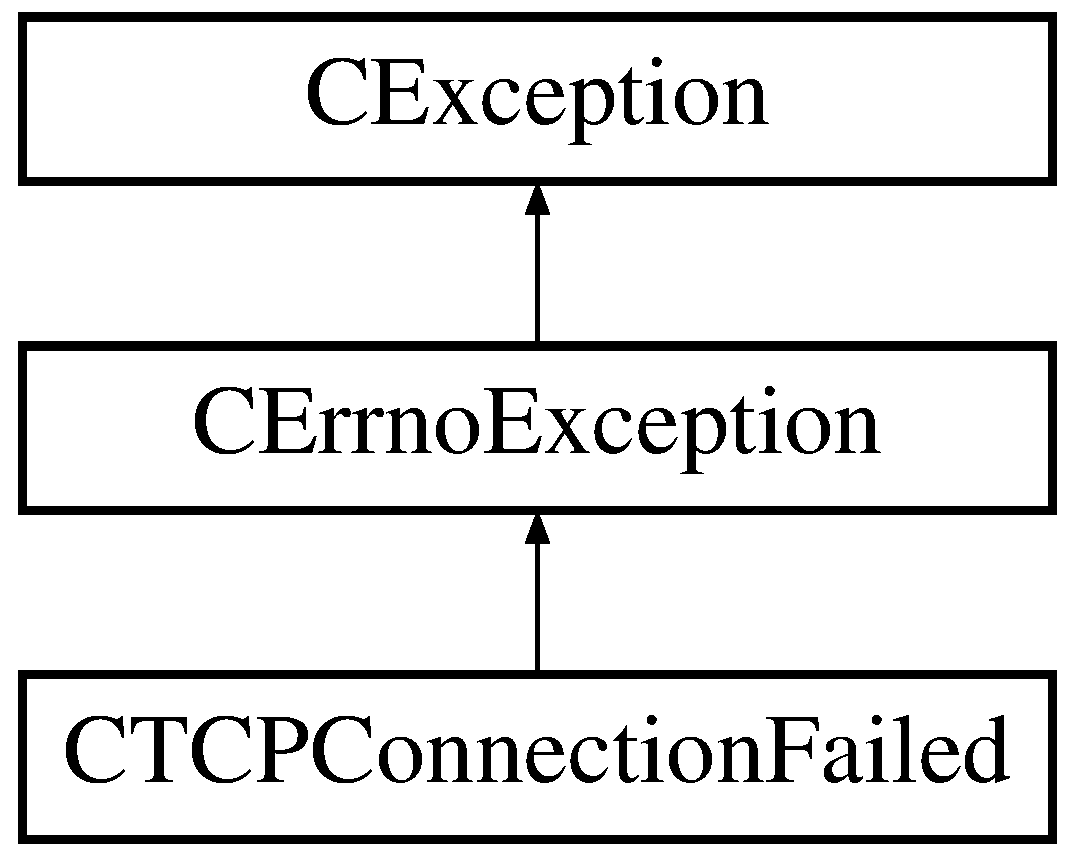
\includegraphics[height=3cm]{classCTCPConnectionFailed}
\end{center}
\end{figure}
\subsection*{Public Methods}
\begin{CompactItemize}
\item 
{\bf CTCPConnection\-Failed} (const string \&host, const string \&service, const char $\ast$p\-Doing)
\item 
{\bf CTCPConnection\-Failed} (const CTCPConnection\-Failed \&rhs)
\item 
{\bf $\sim$CTCPConnection\-Failed} ()
\begin{CompactList}\small\item\em Destructor.\item\end{CompactList}\item 
CTCPConnection\-Failed \& {\bf operator=} (const CTCPConnection\-Failed \&rhs)
\item 
int {\bf operator==} (const CTCPConnection\-Failed \&rhs)
\item 
string {\bf get\-Host} () const
\item 
string {\bf get\-Service} () const
\item 
virtual const char $\ast$ {\bf Reason\-Text} () const
\end{CompactItemize}
\subsection*{Protected Methods}
\begin{CompactItemize}
\item 
void {\bf set\-Host} (const string \&r\-Host)
\item 
void {\bf set\-Service} (const string \&r\-Service)
\end{CompactItemize}
\subsection*{Private Attributes}
\begin{CompactItemize}
\item 
string {\bf m\_\-Host}
\begin{CompactList}\small\item\em Attempted peername.\item\end{CompactList}\item 
string {\bf m\_\-Service}
\begin{CompactList}\small\item\em Attempted connection point port.\item\end{CompactList}\item 
string {\bf m\_\-Reason\-Text}
\begin{CompactList}\small\item\em Reason text is built up here.\item\end{CompactList}\end{CompactItemize}


\subsection{Detailed Description}
Encapsulates a connection failure exception. Since connect(2) reports failure reasons through errno, this classs derives from {\bf CErrno\-Exception} {\rm (p.\,\pageref{classCErrnoException})}. 



Definition at line 297 of file CTCPConnection\-Failed.h.

\subsection{Constructor \& Destructor Documentation}
\index{CTCPConnectionFailed@{CTCPConnection\-Failed}!CTCPConnectionFailed@{CTCPConnectionFailed}}
\index{CTCPConnectionFailed@{CTCPConnectionFailed}!CTCPConnectionFailed@{CTCPConnection\-Failed}}
\subsubsection{\setlength{\rightskip}{0pt plus 5cm}CTCPConnection\-Failed::CTCPConnection\-Failed (const string \& {\em host}, const string \& {\em service}, const char $\ast$ {\em p\-Doing})}\label{classCTCPConnectionFailed_a0}


'Normal constructor' intended to be used to instantiate an object prior to throwing it as an exception.\begin{Desc}
\item[Parameters: ]\par
\begin{description}
\item[{\em 
host}]- Name of the host which to which the connection was attempted \item[{\em 
service}]- Textualized service to which the connection was attempted \item[{\em 
p\-Doing}]- Context information describing what {\bf CSocket} {\rm (p.\,\pageref{classCSocket})} was doing when the exceptional condition was detected. \end{description}
\end{Desc}


Definition at line 298 of file CTCPConnection\-Failed.cpp.\index{CTCPConnectionFailed@{CTCPConnection\-Failed}!CTCPConnectionFailed@{CTCPConnectionFailed}}
\index{CTCPConnectionFailed@{CTCPConnectionFailed}!CTCPConnectionFailed@{CTCPConnection\-Failed}}
\subsubsection{\setlength{\rightskip}{0pt plus 5cm}CTCPConnection\-Failed::CTCPConnection\-Failed (const CTCPConnection\-Failed \& {\em rhs})}\label{classCTCPConnectionFailed_a1}


Copy Constructor. Used by the compiler to create temporaries and by the throw statement to create a copy of the actual exception object to ensure that the exception remains in scope while it travels up the call stack  searching for a handler.\begin{Desc}
\item[Parameters: ]\par
\begin{description}
\item[{\em 
rhs}]- The reference object which is being copy constructed. \end{description}
\end{Desc}


Definition at line 314 of file CTCPConnection\-Failed.cpp.\index{CTCPConnectionFailed@{CTCPConnection\-Failed}!~CTCPConnectionFailed@{$\sim$CTCPConnectionFailed}}
\index{~CTCPConnectionFailed@{$\sim$CTCPConnectionFailed}!CTCPConnectionFailed@{CTCPConnection\-Failed}}
\subsubsection{\setlength{\rightskip}{0pt plus 5cm}CTCPConnection\-Failed::$\sim$CTCPConnection\-Failed ()\hspace{0.3cm}{\tt  [inline]}}\label{classCTCPConnectionFailed_a2}


Destructor.



Definition at line 312 of file CTCPConnection\-Failed.h.

\subsection{Member Function Documentation}
\index{CTCPConnectionFailed@{CTCPConnection\-Failed}!getHost@{getHost}}
\index{getHost@{getHost}!CTCPConnectionFailed@{CTCPConnection\-Failed}}
\subsubsection{\setlength{\rightskip}{0pt plus 5cm}string CTCPConnection\-Failed::get\-Host () const\hspace{0.3cm}{\tt  [inline]}}\label{classCTCPConnectionFailed_a5}




Definition at line 320 of file CTCPConnection\-Failed.h.

References m\_\-Host.\index{CTCPConnectionFailed@{CTCPConnection\-Failed}!getService@{getService}}
\index{getService@{getService}!CTCPConnectionFailed@{CTCPConnection\-Failed}}
\subsubsection{\setlength{\rightskip}{0pt plus 5cm}string CTCPConnection\-Failed::get\-Service () const\hspace{0.3cm}{\tt  [inline]}}\label{classCTCPConnectionFailed_a6}




Definition at line 322 of file CTCPConnection\-Failed.h.

References m\_\-Service.\index{CTCPConnectionFailed@{CTCPConnection\-Failed}!operator=@{operator=}}
\index{operator=@{operator=}!CTCPConnectionFailed@{CTCPConnection\-Failed}}
\subsubsection{\setlength{\rightskip}{0pt plus 5cm}CTCPConnection\-Failed \& CTCPConnection\-Failed::operator= (const CTCPConnection\-Failed \& {\em rhs})}\label{classCTCPConnectionFailed_a3}


Assignment. The functionality is the same as a copy constructor, however the target is a fully constructed object. We protect, therefore against assignment to $\ast$this, and since this is not a constructor, we cannot use initializers to assign our members. \begin{Desc}
\item[Parameters: ]\par
\begin{description}
\item[{\em 
rhs}]- The object we are being assigned to. \end{description}
\end{Desc}


Definition at line 328 of file CTCPConnection\-Failed.cpp.

References m\_\-Host, m\_\-Service, and CErrno\-Exception::operator=().\index{CTCPConnectionFailed@{CTCPConnection\-Failed}!operator==@{operator==}}
\index{operator==@{operator==}!CTCPConnectionFailed@{CTCPConnection\-Failed}}
\subsubsection{\setlength{\rightskip}{0pt plus 5cm}int CTCPConnection\-Failed::operator== (const CTCPConnection\-Failed \& {\em rhs})}\label{classCTCPConnectionFailed_a4}


Equality compare... This is essentially a member by member compare. \begin{Desc}
\item[Parameters: ]\par
\begin{description}
\item[{\em 
rhs}]- the object to which we are being compared. \end{description}
\end{Desc}


Definition at line 342 of file CTCPConnection\-Failed.cpp.

References m\_\-Host, m\_\-Service, and CErrno\-Exception::operator==().\index{CTCPConnectionFailed@{CTCPConnection\-Failed}!ReasonText@{ReasonText}}
\index{ReasonText@{ReasonText}!CTCPConnectionFailed@{CTCPConnection\-Failed}}
\subsubsection{\setlength{\rightskip}{0pt plus 5cm}const char $\ast$ CTCPConnection\-Failed::Reason\-Text () const\hspace{0.3cm}{\tt  [virtual]}}\label{classCTCPConnectionFailed_a7}


Returns a textual string describing the message. This is going to be something like: Failed to connect to host: m\_\-Host on service port m\_\-Service,  {\bf CErrno\-Exception::Reason\-Text}() {\rm (p.\,\pageref{classCErrnoException_a7})}. 

Reimplemented from {\bf CErrno\-Exception} {\rm (p.\,\pageref{classCErrnoException_a7})}.

Definition at line 355 of file CTCPConnection\-Failed.cpp.

References m\_\-Host, m\_\-Reason\-Text, m\_\-Service, and CErrno\-Exception::Reason\-Text().\index{CTCPConnectionFailed@{CTCPConnection\-Failed}!setHost@{setHost}}
\index{setHost@{setHost}!CTCPConnectionFailed@{CTCPConnection\-Failed}}
\subsubsection{\setlength{\rightskip}{0pt plus 5cm}void CTCPConnection\-Failed::set\-Host (const string \& {\em r\-Host})\hspace{0.3cm}{\tt  [inline, protected]}}\label{classCTCPConnectionFailed_b0}




Definition at line 328 of file CTCPConnection\-Failed.h.

References m\_\-Host.\index{CTCPConnectionFailed@{CTCPConnection\-Failed}!setService@{setService}}
\index{setService@{setService}!CTCPConnectionFailed@{CTCPConnection\-Failed}}
\subsubsection{\setlength{\rightskip}{0pt plus 5cm}void CTCPConnection\-Failed::set\-Service (const string \& {\em r\-Service})\hspace{0.3cm}{\tt  [inline, protected]}}\label{classCTCPConnectionFailed_b1}




Definition at line 330 of file CTCPConnection\-Failed.h.

References m\_\-Service.

\subsection{Member Data Documentation}
\index{CTCPConnectionFailed@{CTCPConnection\-Failed}!m_Host@{m\_\-Host}}
\index{m_Host@{m\_\-Host}!CTCPConnectionFailed@{CTCPConnection\-Failed}}
\subsubsection{\setlength{\rightskip}{0pt plus 5cm}string CTCPConnection\-Failed::m\_\-Host\hspace{0.3cm}{\tt  [private]}}\label{classCTCPConnectionFailed_o0}


Attempted peername.



Definition at line 301 of file CTCPConnection\-Failed.h.

Referenced by get\-Host(), operator=(), operator==(), Reason\-Text(), and set\-Host().\index{CTCPConnectionFailed@{CTCPConnection\-Failed}!m_ReasonText@{m\_\-ReasonText}}
\index{m_ReasonText@{m\_\-ReasonText}!CTCPConnectionFailed@{CTCPConnection\-Failed}}
\subsubsection{\setlength{\rightskip}{0pt plus 5cm}string CTCPConnection\-Failed::m\_\-Reason\-Text\hspace{0.3cm}{\tt  [private]}}\label{classCTCPConnectionFailed_o2}


Reason text is built up here.



Definition at line 303 of file CTCPConnection\-Failed.h.

Referenced by Reason\-Text().\index{CTCPConnectionFailed@{CTCPConnection\-Failed}!m_Service@{m\_\-Service}}
\index{m_Service@{m\_\-Service}!CTCPConnectionFailed@{CTCPConnection\-Failed}}
\subsubsection{\setlength{\rightskip}{0pt plus 5cm}string CTCPConnection\-Failed::m\_\-Service\hspace{0.3cm}{\tt  [private]}}\label{classCTCPConnectionFailed_o1}


Attempted connection point port.



Definition at line 302 of file CTCPConnection\-Failed.h.

Referenced by get\-Service(), operator=(), operator==(), Reason\-Text(), and set\-Service().

The documentation for this class was generated from the following files:\begin{CompactItemize}
\item 
{\bf CTCPConnection\-Failed.h}\item 
{\bf CTCPConnection\-Failed.cpp}\end{CompactItemize}
